\chapter{Entwurf}
\thispagestyle{standard}
\pagestyle{standard}
\renewcommand{\footrulewidth}{0.4pt}
\lfoot{\small Refik Kerimi}

In diesem Kapitel wird das Muster und die Anforderungen bzw. die Umsetzung der \aclp{PWA} (\acs{PWA}) im Allgemeinen betrachtet.


\section{Übersicht PWA}\label{sub:Übersicht PWA}
%https://developers.google.com/web/ilt/pwa/introduction-to-progressive-web-app-architectures
% Die Architektur soll beschrieben weden
Im Gegensatz zur \acl{NA} (\acs{NA}) ist die \acl{PWA} (\acs{PWA}) eine \acl{SC} (\acs{SC}) Architektur, diese wird nicht auf dem Client gespeichert sondern es wird über den Browser und das HTTPS-Protokoll zwischen Client und Server kommuniziert. Im Unterschied zu HTTP ist, wie in Abbildung \ref{fig:HTTP_HTTPS} zu sehen, die Verbindung verschlüsselt.

\begin{figure}[h]
	\centering
	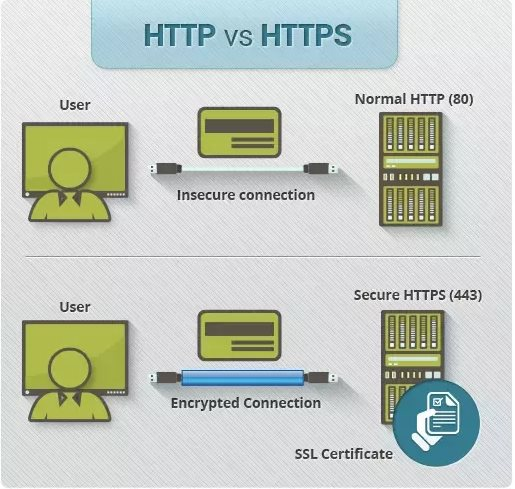
\includegraphics[width=6cm]{BilderAllgemein/HTTP_HTTPS}\medskip
	\caption{Unterschied HTTP/HTTPS \cite{HTTPS}}
	\label{fig:HTTP_HTTPS}
\end{figure}

Dies hat den Vorteil das die Applikation sowie die Updates wie schon in Kapitel \ref{chap:PWAvs.NativeApplikationvsWeb Applikation} erwähnt nicht downgeloaded und installiert werden müssen, das wird alles Server seitig erledigt. 

\newpage

\section{Anforderungsanalyse}\label{sub:Anforderungsanalyse}
Die zu entwickelnde Smart Home Applikation muss das verhalten einer \acs{PWA} aufweisen. Das heißt es müssen die Attribute aus Kapitel \ref{chap:ProgressiveWebapplikationen} eingebaut werden und danach im Kapitel \ref{chap:Funktionstest} getestet werden. Außerdem sollen auch APIs entwickelt werden die es möglich machen mit Services von Drittanbietern die Temperatur zu regeln, mit Hilfe von Geolocation API soll der Standort ermittelt werden um das Garagentor automatisch öffnen zu können. Auch soll das Steuern der Beleuchtung möglich sein. Diese Applikation soll Offline so weit es geht Verwendbar sein. Die Anwendung muss Plattformunabhängig und Responsive sein.


